\section{The \name{} System}\label{sec:solution}

In this section, we introduce \name{}, a general and effective GraphRAG solution designed to handle a wide range of graph questions. \name{} automatically classifies and decomposes user questions into a sequence of basic sub-questions. For each sub-question, it generates an appropriate Cypher query with adaptive prompting and self-correction mechanisms to retrieve relevant information. The responses to these sub-questions are then aggregated and fed into the LLM to produce a final answer.

As depicted in~\autoref{fig:workflow}, \name{} comprises five main stages: \textit{question categorization}, \textit{question decomposition}, \textit{Cypher query generation}, \textit{query execution} and \textit{context formation}. In the following, we describe each stage in detail. The full prompt used in each module is provided in \autoref{sec:prompts_appendix}.

\stitle{Question categorization.} Given a user question, \name{} prompts the LLM to classify it as either a \textit{basic} or \textit{nested} question by providing clear definitions of the basic question patterns along with few-shot examples. A basic question directly corresponds to one of the four defined patterns, whereas a nested question represents a composition of multiple basic questions. If the input is identified as a basic question, the LLM is also required to specify its exact pattern type. For instance, the question “\textit{Who developed universal gravitation?}” is categorized as a basic question with the pattern $\langle s, p, * \rangle$.


\begin{figure*}[!t]
	\centering
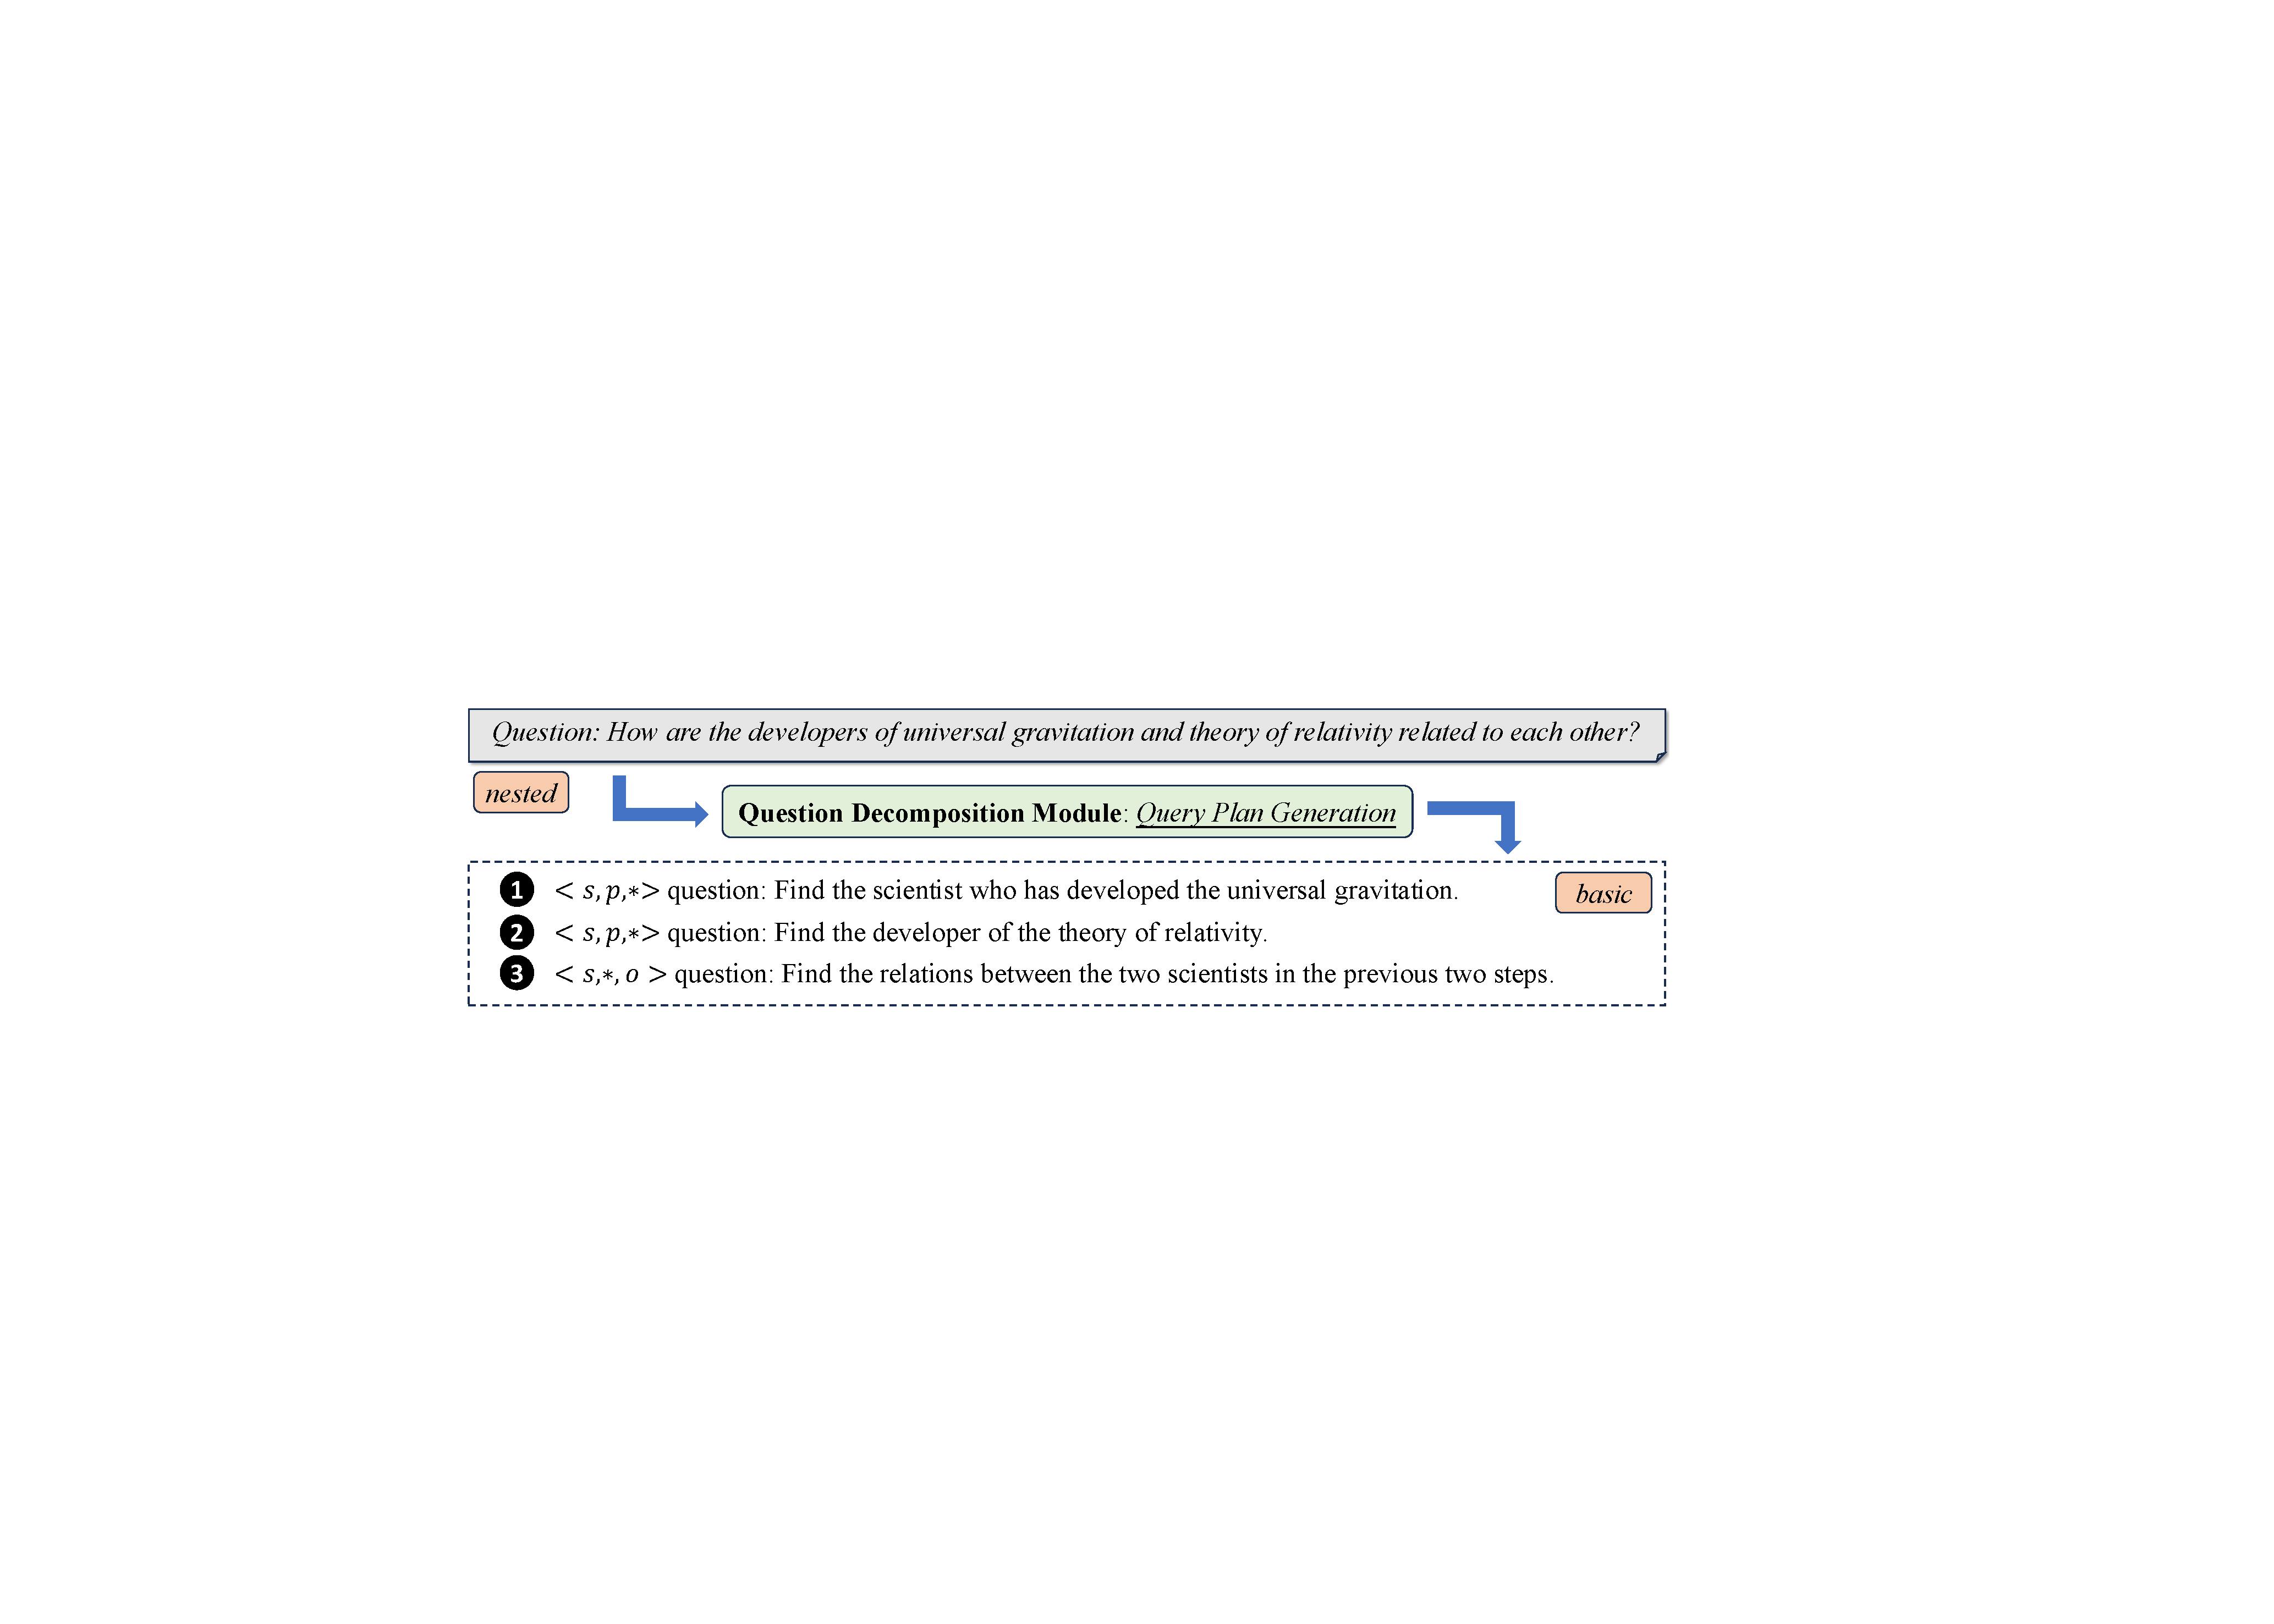
\includegraphics[width=0.9\textwidth]{figures/question_decompose.pdf}
	% \vspace{-2mm}
	\caption{An example of the question decomposition in \name{}.}
\label{fig:question_decompose}
	 \vspace{-4mm}
\end{figure*}

\stitle{Question decomposition.} For nested questions, \name{} prompts the LLM to decompose the complex input into a sequence of basic questions. However, it is often not possible to generate concrete sub-questions without first obtaining intermediate results. For instance, given the question “\textit{How are the developers of universal gravitation and the theory of relativity related to each other?}”, we cannot form the sub-question “\textit{How are Isaac Newton and Albert Einstein related?}” until we have identified these individuals as the developers in earlier steps. Therefore, rather than asking the LLM to generate fully instantiated sub-questions, we prompt it to produce a \textit{query plan}, where each step describes a specific sub-question to be resolved. An example is shown in~\autoref{fig:question_decompose}, where the third step in the query plan is: “\textit{Find the relations between the two scientists identified in the previous two steps},” rather than a fully specified question.


\stitle{Cypher query generation.} Once the query plan is constructed with descriptive steps, \name{} instantiates a concrete basic question for each step before execution. At this stage, the LLM is given the full query plan along with all previously generated sub-questions and their responses, and is asked to generate a concrete question for the current step. \name{} then adaptively prompts the LLM to produce a faithful Cypher query by providing the graph schema (i.e., entity and relation types) and task-specific instructions. While the full schemas of large RDF knowledge graphs (e.g., Wikidata and Freebase) may exceed the LLM's context length, prior work~\cite{cypherbench,rdf2property} has proposed techniques to convert RDF graphs into multiple smaller property graphs with manageable schema sizes. Since each of the four basic question patterns targets different components of a knowledge graph fact triple, as discussed in~\autoref{sec:question_categorization}, we observe that they necessitate \textit{distinct graph traversal strategies}.

\begin{wraptable}{r}{0.45\textwidth}
\centering
\caption{Correspondence from graph question patterns to specific graph traversal strategies.}
\label{tab:traversal_patterns}
\resizebox{0.45\textwidth}{!}{%
\begin{tabular}{@{}cc@{}}
\toprule
\textbf{Question Pattern} & \textbf{Graph Traversal Strategy}         \\ \midrule
$\langle s,*,* \rangle$ & BFS neighbor expansion    \\
$\langle s,p,* \rangle$ & meta-path guided walk      \\
$\langle s,*,o \rangle$ & top-k shortest paths             \\
$\langle s,p,o \rangle$ & top-k constrained shortest paths \\ \bottomrule
\end{tabular}%
}
\end{wraptable}

In~\autoref{tab:traversal_patterns}, we summarize the graph traversal strategies employed for each basic question pattern. Specifically, $\langle s,*,* \rangle$ questions aim to retrieve general information and are best handled via \textit{BFS neighbor expansion}, using queries such as \texttt{``MATCH (s)-[p]->(o) RETURN p, o''}. This approach efficiently captures the immediate neighborhood of the subject $s$ by gathering its one-hop neighbors and directly connected relations. For $\langle s,p,* \rangle$ questions, where the relation $p$ is explicitly defined, we prompt the LLM to generate \textit{concrete meta-paths} that connect the subject $s$ to the target entity $o$. A typical Cypher query for this pattern is of the form \texttt{``MATCH (s)-[p1]->(o1)-[p2]->...->(on) WHERE... RETURN on''}, where \texttt{n} denotes the number of hops in the relational chain and $p_1...p_n$ constitute $p$. This guided traversal not only accurately locates the answer but also reduces unnecessary context. For $\langle s,*,o \rangle$ and $\langle s,p,o \rangle$ questions, which inquire about the relations, we generate Cypher queries that perform a \textit{top-$k$ shortest paths} search to identify all relevant paths between $s$ and $o$, using queries such as \texttt{``MATCH P = SHORTEST k (s)-[*]->(o) RETURN P''}. In the case of $\langle s,p,o \rangle$ questions, where $p$ is known, we further prompt the LLM to apply filtering clauses (e.g., \texttt{``WHERE''}) to ensure that only paths matching $p$ are returned. Beyond shortest-paths, \name{} can also be extended to use random walk methods such as DeepWalk~\cite{deepwalk} and Node2Vec~\cite{node2vec} to uncover meaningful reasoning paths.


\stitle{Query execution.} After the LLM generates a concrete, executable Cypher query for each basic question, \name{} executes the query asynchronously over the underlying graph database. However, even with clear specifications and few-shot examples tailored to each basic question pattern, the LLM may still generate erroneous Cypher queries—such as those with incorrect syntax or nonexistent relations—which can lead to execution errors or empty results. To address this, \name{} incorporates a \textit{self-correction} mechanism that enables the LLM to automatically detect and refine faulty queries upon failure. Specifically, \name{} captures the execution error and sends it back to the LLM along with prior responses to prompt correction. Empirically, we find that setting the maximum number of retries to 3 strikes a good balance between quality and efficiency.


\stitle{Context formation.} Based on the results of each Cypher query from the previous stage, \name{} assembles a complete context to enable the LLM to generate a high-quality response. In addition to task-specific prompts, the core components of this context are the entity and relation tables. The entity table lists all attributes of the retrieved entities (e.g., node type and description), while the relation table aggregates all existing relations and their attributes between each pair of entities. Together, these two tables form the essential context that contains all necessary information to answer the question. Furthermore, for $\langle s, *, o \rangle$ and $\langle s, p, o \rangle$-type questions, we also include additional complete reasoning paths between the question entities to better demonstrate their interconnections. Finally, once \name{} completes all steps in the query plan, it compiles all sub-questions, their corresponding responses, and the original user question to prompt the LLM to generate a final summary.


% In this section, we first present the workflow of \name{}, detailing its process for automatically categorizing and decomposing user questions and generating responses. We then discuss how \name{} constructs an executable traversal plan for each question type and organizes the retrieved information into a structured context during traversal execution.

% \stitle{Workflow.} As shown in \autoref{fig:workflow}, \name{} adaptively selects the appropriate graph traversal method based on the input question and executes the traversal operations through a unified interface to the backend execution engine. Specifically, \name{} follows these steps to answer a user query.

% \circled{1} \textit{Question Categorization:} Given a graph-based question, \name{} prompts the judger LLM to classify it into one of the predefined categories by providing definitions and few-shot examples, as detailed in \autoref{tab:question_description}. The prompt used for classification is provided in \autoref{sec:prompts_classification_appendix}. The judger LLM outputs the question type, which is then used to generate concrete traversal operations in the next step.

% \circled{2} \textit{Traversal Plan Generation:} \name{} extracts anchor entities and potential relation constraints based on the question type. It then fills the extracted keywords into predefined templates for $\langle s, *, * \rangle$ and $\langle s, *, o \rangle$ questions or invokes the generator LLM to construct concrete reasoning paths for $\langle s, p, * \rangle$ and $\langle s, p, o \rangle$ questions.

% \circled{3} \textit{Traversal Execution:} With an executable traversal plan, \name{} interfaces with an underlying Neo4j~\cite{neo4j} graph database and submits the plan as a Cypher query. This query initiates graph traversal starting from the anchor entity ($s$) and, if applicable, reaching the target entity ($o$), depending on the question type.

% \circled{4} \textit{Context Formation:} Once relevant graph entities and relations are retrieved, \name{} organizes the results into structured formats, such as entity and relation tables for $\langle s, *, * \rangle$ and $\langle s, p, * \rangle$ questions, and reasoning path lists for $\langle s, *, o \rangle$ and $\langle s, p, o \rangle$ questions.

% \circled{5} \textit{Answer Generation:} Finally, the structured context is fed to the generator LLM, which synthesizes a final response grounded in the retrieved graph knowledge.

% \stitle{Traversal templates and output formats.} For $\langle s, *, * \rangle$ questions, \name{} follows the approach used in MS\_GraphRAG and LightRAG, locating the anchor entities in the graph, gathering their one-hop neighbors, and returning two tables (i.e., an entity table and a relation table) as the retrieved context. For $\langle s, p, * \rangle$ questions, \name{} provides the LLM with a detailed graph schema, including entity and relation definitions and how different entity types interconnect. It then prompts the LLM to generate reasoning paths based on the schema and the specific input question. \name{} follows the generated reasoning path and retrieves the traversal path from the anchor entity ($s$) to the answer ($o$), along with the entity and relation tables. Unlike RoG, which requires instruction-tuning on the LLM, \name{} avoids fine-tuning, offering greater ease of use. For $\langle s, *, o \rangle$ questions, \name{} extracts the two anchor entities ($s$ and $o$) and executes the top-$k$ shortest paths algorithm on the graph. The results are structured as $k$ paths in a list format (\texttt{entity$\rightarrow$relation$\rightarrow$...$\rightarrow$entity}). Finally, for $\langle s, p, o \rangle$ questions, \name{} extracts both anchor entities ($s$ and $o$) along with the constraints for path matching ($p$). It then performs constrained path matching between the two entities and retrieves the top-$k$ shortest paths that satisfy the constraints. The retrieved paths are presented as multiple path lists, illustrating examples of relationships under the specified constraints.
